\documentclass[12pt,a4paper]{article}

% ============================================================================
% PACKAGES
% ============================================================================
\usepackage[utf8]{inputenc}
\usepackage[T1]{fontenc}
\usepackage{lmodern}
\usepackage[margin=2.5cm]{geometry}
\usepackage{graphicx}
\usepackage{xcolor}
\usepackage{tikz}
\usepackage{pgfplots}
\usepackage{pgfgantt}
\usepackage{booktabs}
\usepackage{array}
\usepackage{multirow}
\usepackage{longtable}
\usepackage{hyperref}
\usepackage{fancyhdr}
\usepackage{titlesec}
\usepackage{tcolorbox}
\usepackage{listings}
\usepackage{caption}
\usepackage{amsmath}
\usepackage{amssymb}
\usepackage{enumitem}
\usepackage{tabularx}
\usepackage{float}
\usepackage{microtype}

% ============================================================================
% CONFIGURATION
% ============================================================================
\pgfplotsset{compat=1.18}
\usetikzlibrary{shapes.geometric, arrows.meta, positioning, calc, decorations.pathreplacing, patterns, shadows, fit, backgrounds}

% Colors
\definecolor{qblue}{RGB}{0, 100, 200}
\definecolor{qpurple}{RGB}{128, 0, 200}
\definecolor{qcyan}{RGB}{0, 180, 200}
\definecolor{qgreen}{RGB}{0, 180, 100}
\definecolor{qorange}{RGB}{255, 140, 0}
\definecolor{qred}{RGB}{220, 50, 50}
\definecolor{darkbg}{RGB}{30, 30, 40}
\definecolor{codebg}{RGB}{245, 245, 250}
\definecolor{crisis}{RGB}{200, 30, 30}
\definecolor{resolved}{RGB}{30, 150, 80}
\definecolor{feature}{RGB}{30, 80, 200}

% Hyperref setup
\hypersetup{
    colorlinks=true,
    linkcolor=qblue,
    urlcolor=qpurple,
    citecolor=qgreen,
    pdftitle={Quillon Graph: Project Status Report v4},
    pdfauthor={Q-NarwhalKnight Development Team}
}

% Header/Footer
\pagestyle{fancy}
\fancyhf{}
\fancyhead[L]{\textsc{Quillon Graph}}
\fancyhead[R]{\textsc{Project Report v4 --- Operation Twelve Gauge}}
\fancyfoot[C]{\thepage}
\renewcommand{\headrulewidth}{0.4pt}

% Title formatting
\titleformat{\section}{\Large\bfseries\color{qblue}}{\thesection}{1em}{}
\titleformat{\subsection}{\large\bfseries\color{qpurple}}{\thesubsection}{1em}{}
\titleformat{\subsubsection}{\normalsize\bfseries\color{qcyan}}{\thesubsubsection}{1em}{}

% Listing style
\lstset{
    backgroundcolor=\color{codebg},
    basicstyle=\ttfamily\small,
    breaklines=true,
    frame=single,
    rulecolor=\color{qblue!30},
    numbers=left,
    numberstyle=\tiny\color{gray},
    keywordstyle=\color{qblue}\bfseries,
    commentstyle=\color{qgreen},
    stringstyle=\color{qorange},
}

% Custom boxes
\tcbuselibrary{skins,breakable}

\newtcolorbox{milestone}{
    colback=qblue!5,
    colframe=qblue,
    title={Milestone Achieved},
    fonttitle=\bfseries,
    rounded corners,
    boxrule=1pt,
}

\newtcolorbox{crisisbox}{
    colback=qred!5,
    colframe=qred,
    fonttitle=\bfseries,
    rounded corners,
    boxrule=1pt,
}

\newtcolorbox{statbox}{
    colback=qgreen!5,
    colframe=qgreen,
    fonttitle=\bfseries,
    rounded corners,
    boxrule=1pt,
}

\newtcolorbox{futurebox}{
    colback=qpurple!5,
    colframe=qpurple,
    title={Future Development},
    fonttitle=\bfseries,
    rounded corners,
    boxrule=1pt,
}

% ============================================================================
% DOCUMENT
% ============================================================================
\begin{document}

% Title Page
\begin{titlepage}
    \centering
    \vspace*{1.5cm}

    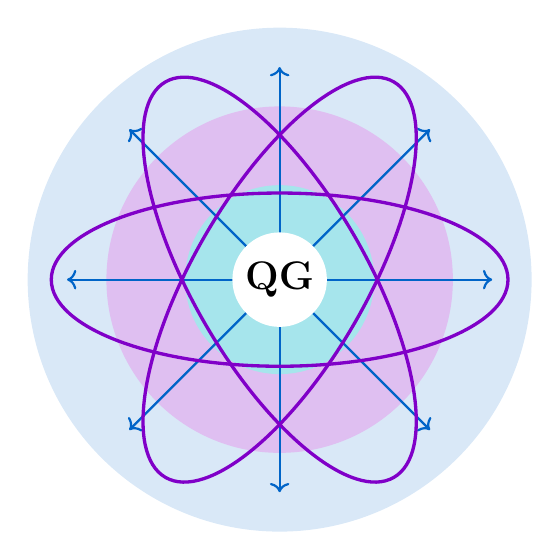
\begin{tikzpicture}
        % Quantum symbol background
        \fill[qblue!15] (0,0) circle (3.2cm);
        \fill[qpurple!25] (0,0) circle (2.2cm);
        \fill[qcyan!35] (0,0) circle (1.2cm);

        % DAG lattice representation
        \foreach \angle in {0,45,90,135,180,225,270,315} {
            \draw[qblue, thick, ->] (0,0) -- (\angle:2.7cm);
        }
        \draw[qpurple, very thick] (0,0) ellipse (2.9cm and 1.1cm);
        \draw[qpurple, very thick, rotate=60] (0,0) ellipse (2.9cm and 1.1cm);
        \draw[qpurple, very thick, rotate=120] (0,0) ellipse (2.9cm and 1.1cm);

        % Center node
        \fill[white] (0,0) circle (0.6cm);
        \node at (0,0) {\Large\textbf{QG}};
    \end{tikzpicture}

    \vspace{1.2cm}

    {\Huge\bfseries\color{qblue} Quillon Graph}\\[0.4cm]
    {\Large\color{qpurple} Project Status Report v4}\\[0.3cm]
    {\large\color{qcyan} Operation Twelve Gauge (Continued)}\\[0.6cm]
    {\large\itshape February--April 2026: From Crisis to Innovation}

    \vspace{1.5cm}

    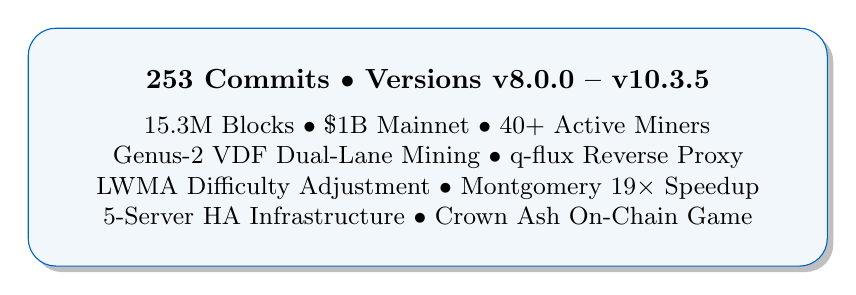
\begin{tikzpicture}
        \node[draw=qblue, rounded corners=10pt, fill=qblue!5, inner sep=15pt, drop shadow] {
            \begin{minipage}{0.75\textwidth}
                \centering
                \textbf{253 Commits $\bullet$ Versions v8.0.0 -- v10.3.5}\\[5pt]
                \small
                15.3M Blocks $\bullet$ \$1B Mainnet $\bullet$ 40+ Active Miners\\
                Genus-2 VDF Dual-Lane Mining $\bullet$ q-flux Reverse Proxy\\
                LWMA Difficulty Adjustment $\bullet$ Montgomery 19$\times$ Speedup\\
                5-Server HA Infrastructure $\bullet$ Crown Ash On-Chain Game
            \end{minipage}
        };
    \end{tikzpicture}

    \vfill

    {\large April 15, 2026}\\[0.5cm]
    \texttt{https://quillon.xyz}

\end{titlepage}

% Table of Contents
\tableofcontents
\newpage

% ============================================================================
% SECTION 1: EXECUTIVE SUMMARY
% ============================================================================
\section{Executive Summary}

This report covers the most intense period of Quillon Graph (Q-NarwhalKnight) development: February 15 through April 15, 2026. During these two months, the project transitioned from pre-launch preparation to a live, \$1B-market-cap mainnet, survived multiple critical crises, and delivered breakthrough innovations in CPU-fair mining.

\begin{statbox}
\textbf{Period Statistics (Feb 15 -- Apr 15, 2026)}\\[10pt]
\begin{tabular}{@{}ll@{\hspace{2cm}}ll@{}}
\textbf{Total Commits:} & 253 & \textbf{Version Range:} & v8.0.0 -- v10.3.5 \\
\textbf{Network Height:} & 15.3M blocks & \textbf{Block Rate:} & 3.37 bps (pre-LWMA) \\
\textbf{Active Miners:} & 40+ & \textbf{Hash Rate:} & 11.38 GH/s \\
\textbf{Total Mined:} & 396{,}162 / 21M QUG & \textbf{Infrastructure:} & 5 servers \\
\textbf{Peak Day Commits:} & 26 (Mar 8) & \textbf{Longest Session:} & 18 hours \\
\textbf{Critical Incidents:} & 11 & \textbf{Resolved:} & 11/11 \\
\end{tabular}
\end{statbox}

\subsection{Period Highlights}

\begin{itemize}
    \item \textbf{Mainnet Launch (Feb 22):} Genesis block produced at 12:00 UTC with mainnet2026.2 network ID, emission rate of 2{,}625{,}000 QUG/year
    \item \textbf{Connection Pileup Crisis (Mar 4):} 38{,}000 TCP connections, 87\% 503 error rate resolved with q-flux reverse proxy
    \item \textbf{q-flux Development (Mar 5--8):} Custom high-performance reverse proxy built from scratch, deployed on Epsilon
    \item \textbf{Emergency 18-Hour Session (Apr 13--14):} Balance reorg handler discovered as root cause of balance loss; 5 critical bugs fixed
    \item \textbf{Genus-2 VDF Mining (Apr 14--15):} Dual-lane BLAKE3/VDF mining protocol with 50/50 reward split for CPU fairness
    \item \textbf{Montgomery Optimization (Apr 15):} 19$\times$ VDF speedup via CIOS Montgomery multiplication (521$\mu$s $\to$ 200$\mu$s per doubling)
    \item \textbf{LWMA Difficulty (Apr 13):} Linearly Weighted Moving Average difficulty adjustment activated at height 14{,}900{,}000
    \item \textbf{Dragon Ball Collaboration (Apr 9--10):} FPGA/ASIC mining partnership with Dragon Ball team (Kintex-7 XC7K355T)
\end{itemize}

% ============================================================================
% SECTION 2: TIMELINE & MILESTONES
% ============================================================================
\section{Timeline and Milestones}

\subsection{Chronological Overview}

The two-month period divides naturally into five phases: launch preparation, initial mining, infrastructure crisis, stabilization, and innovation.

\subsection{Project Gantt Chart}

\begin{center}
\begin{ganttchart}[
    hgrid,
    vgrid,
    x unit=0.23cm,
    y unit chart=0.55cm,
    y unit title=0.7cm,
    title height=1,
    bar height=0.5,
    bar label font=\scriptsize,
    group label font=\bfseries\scriptsize,
    milestone label font=\scriptsize\color{qred},
    title label font=\scriptsize\bfseries,
    canvas/.append style={fill=gray!5},
    bar/.append style={fill=qblue!60, draw=qblue},
    bar incomplete/.append style={fill=qblue!20},
    group/.append style={fill=qpurple!40, draw=qpurple},
    milestone/.append style={fill=qred, draw=qred},
]{1}{60}

    \gantttitle{February}{13}
    \gantttitle{March}{31}
    \gantttitle{April}{16} \\
    \gantttitlelist{16,...,28}{1}
    \gantttitlelist{1,...,31}{1}
    \gantttitlelist{1,...,16}{1} \\

    % Phase 1: Launch Prep
    \ganttgroup{Launch Preparation}{1}{7} \\
    \ganttbar{v8.0.0 Crate Updates}{4}{4} \\
    \ganttbar{Mainnet 2026.2 Config}{1}{7} \\
    \ganttmilestone{Genesis (Feb 22)}{7} \\

    % Phase 2: Initial Mining
    \ganttgroup{Initial Mining}{7}{19} \\
    \ganttbar{v8.1--v8.9 Mining Infra}{7}{17} \\
    \ganttbar{Miner Bandwidth Opt.}{17}{19} \\

    % Phase 3: Infrastructure Crisis
    \ganttgroup{Infrastructure Crisis}{17}{22} \\
    \ganttbar[bar/.append style={fill=qred!60}]{38K Connection Pileup}{17}{17} \\
    \ganttbar[bar/.append style={fill=qorange!60}]{q-flux Development}{19}{22} \\
    \ganttbar[bar/.append style={fill=qred!60}]{Port 8080 Crash-Loop}{22}{22} \\
    \ganttmilestone{q-flux Deployed (Mar 8)}{22} \\

    % Phase 4: Stabilization
    \ganttgroup{Stabilization}{22}{44} \\
    \ganttbar{v9.x Miner Optimizations}{26}{28} \\
    \ganttbar{Starship Compute}{22}{25} \\
    \ganttbar{GPU Mining + OpenCL}{40}{42} \\
    \ganttbar{Crown Ash Game}{42}{42} \\
    \ganttbar{Windows Cross-Compile}{42}{42} \\

    % Phase 5: Innovation
    \ganttgroup{Innovation Period}{44}{60} \\
    \ganttbar[bar/.append style={fill=qred!60}]{DEX Decimal Crisis}{49}{49} \\
    \ganttbar[bar/.append style={fill=qred!60}]{kill -9 Corrupt Blocks}{51}{53} \\
    \ganttbar{Height Stall Fix}{53}{54} \\
    \ganttbar{Dragon Ball FPGA}{54}{55} \\
    \ganttbar[bar/.append style={fill=qred!60}]{Pruning Bug Fix}{57}{57} \\
    \ganttbar[bar/.append style={fill=qred!70}]{EMERGENCY 18h Session}{58}{58} \\
    \ganttbar[bar/.append style={fill=qgreen!60}]{Genus-2 VDF Mining}{58}{59} \\
    \ganttbar[bar/.append style={fill=qgreen!60}]{Montgomery 19$\times$}{60}{60} \\
    \ganttbar[bar/.append style={fill=qgreen!60}]{Checkpoint Sync}{60}{60} \\

\end{ganttchart}
\end{center}

\subsection{Commit Activity Heatmap}

The busiest days correlate directly with crisis response and major feature launches:

\begin{center}
\begin{tabular}{@{}llrl@{}}
\toprule
\textbf{Date} & \textbf{Event} & \textbf{Commits} & \textbf{Category} \\
\midrule
Mar 8 & q-flux reverse proxy + Epsilon deployment & 26 & Infrastructure \\
Mar 7 & q-flux/q-queue development sprint & 25 & Infrastructure \\
Apr 14 & EMERGENCY session + VDF dual-lane & 23 & Crisis + Feature \\
Mar 10 & Starship Endgame compute orchestrator & 20 & Feature \\
Mar 28 & Crown Ash + Windows cross-compile & 19 & Feature \\
Apr 7 & VDF verification + turbo sync fixes & 15 & Bug Fix \\
Mar 27 & GPU mining OpenCL + Tor rustls & 12 & Feature \\
Mar 4 & Connection pileup crisis response & 12 & Crisis \\
\bottomrule
\end{tabular}
\end{center}

% ============================================================================
% SECTION 3: CRITICAL INCIDENTS
% ============================================================================
\section{Critical Incidents and Resolution}

Eleven critical incidents occurred during this period. Every one was resolved without permanent data loss. The table below summarizes each incident, followed by detailed analysis of the most significant ones.

\begin{center}
\small
\begin{longtable}{@{}p{2.8cm}lp{3.5cm}p{3.5cm}l@{}}
\toprule
\textbf{Incident} & \textbf{Date} & \textbf{Root Cause} & \textbf{Resolution} & \textbf{Impact} \\
\midrule
\endhead
Emission 34$\times$ Overshoot & Feb 9 & \texttt{BASE\_ANNUAL\_EMISSION} had 3 extra zeros & Corrected constant, wired \texttt{add\_block()} & HIGH \\
\midrule
RocksDB OOM (26.9GB) & Feb 19 & Block cache auto-sized to 1/3 RAM (16GB) & \texttt{ROCKSDB\_BLOCK\_CACHE\_MB=4096} & HIGH \\
\midrule
Height Regression & Feb 19 & Fast recovery threshold $>$10K; \texttt{save\_safe\_floor()} used non-synced put & Lowered threshold to $>$1K; use \texttt{put\_sync()} & HIGH \\
\midrule
Block-Pack OOM & Mar 6 & Unbounded \texttt{tokio::spawn} for block-pack; 10GB+ allocations & Semaphore(4), 200-block cap per response & CRITICAL \\
\midrule
Connection Pileup & Mar 4 & 38K TCP connections, mining endpoint blocking & Non-blocking challenge lock, q-flux proxy & CRITICAL \\
\midrule
Port 8080 Collision & Mar 8 & Ephemeral port range included 8080; TCP self-connection & \texttt{ip\_local\_port\_range=32768 60999} & HIGH \\
\midrule
DEX Decimal Mismatch & Apr 4 & 8-decimal reserves caused trillion-dollar prices & MIN\_POOL\_RESERVE=$10^{22}$, deepest pool selection & HIGH \\
\midrule
kill -9 Corrupt Blocks & Apr 6 & 180 corrupt blocks from forced kill on Epsilon & Post-scan cleanup, turbo sync refill & HIGH \\
\midrule
Height Atomic Stall & Apr 8 & \texttt{fetch\_max} not used in 4 dedup paths & \texttt{fetch\_max} in all paths + reconciliation & HIGH \\
\midrule
Balance Reorg Handler & Apr 14 & \texttt{saturating\_sub} zeros balances when old\_reward $>$ balance & Disabled handler with \texttt{if false} & CRITICAL \\
\midrule
Pruning Bug & Apr 12 & Early blocks (0--1.6M) deleted by aggressive pruning & Pruning disabled, gap detection for sync & HIGH \\
\bottomrule
\end{longtable}
\end{center}

\subsection{Detailed Analysis: Connection Pileup Crisis (March 4)}

\begin{crisisbox}
\textbf{Severity:} CRITICAL --- 87\% of mining requests failed\\
\textbf{Duration:} 6 hours from detection to resolution\\
\textbf{Root Cause:} The \texttt{/api/v1/mining/challenge} endpoint held a write lock during block production. When 500+ miners polled simultaneously, each request queued behind the lock, creating a cascade of 38{,}000 TCP connections.
\end{crisisbox}

The resolution came in three stages:
\begin{enumerate}
    \item \textbf{Immediate (v8.9.8):} Replaced write lock with non-blocking \texttt{try\_lock}; miners receive cached challenge on contention
    \item \textbf{Short-term (v9.0.1):} Reduced miner bandwidth from 111 KB/s to 2--5 KB/s per miner
    \item \textbf{Permanent (q-flux):} Built a custom reverse proxy with connection pooling, upstream semaphore (256 max in-flight per worker), and health-based failover
\end{enumerate}

\subsection{Detailed Analysis: Emergency 18-Hour Session (April 13--14)}

\begin{crisisbox}
\textbf{Severity:} CRITICAL --- user reported balance loss on \$1B mainnet\\
\textbf{Duration:} 18 continuous hours\\
\textbf{Bugs Found:} 5 (2 critical, 2 high, 1 medium)
\end{crisisbox}

The session began when the project operator reported that QUG balances had dropped unexpectedly. Investigation revealed cascading failures:

\begin{enumerate}
    \item \textbf{Balance Reorg Handler (CRITICAL):} The \texttt{perform\_balance\_reorg()} function used \texttt{saturating\_sub} to remove old rewards during chain reorganization. When \texttt{old\_reward > current\_balance} (common after DEX swaps reduced the balance), the subtraction zeroed the account. This bug had been present since v0.9.31 but only triggered under specific reorg conditions.

    \item \textbf{DEX Double Deduction (CRITICAL):} The swap handler both deducted directly from RocksDB AND submitted a consensus transaction that deducted again. Every swap lost 2$\times$ the intended amount.

    \item \textbf{Ghost Balance on Startup (MEDIUM):} A 10-second window between RocksDB load and authority sync showed stale values, causing user confusion.

    \item \textbf{q-flux Cluster Failover (HIGH):} No failover peers configured; all miners lost connection during Epsilon restarts.

    \item \textbf{Persistent Dedup (HIGH):} Balance deduplication cache did not survive restarts, causing duplicate processing.
\end{enumerate}

Resolution: The reorg handler was disabled entirely (wrapped in \texttt{if false}). Balances were restored from Beta (the authority node) via a one-time P2P sync to all 274 wallets. The DEX double-deduction was fixed by removing the direct deduction path.

% ============================================================================
% SECTION 4: TECHNICAL ACHIEVEMENTS
% ============================================================================
\section{Technical Achievements}

\subsection{Genus-2 Jacobian VDF (2{,}250 Lines)}

The most significant technical achievement of the period is the implementation of a Verifiable Delay Function based on repeated doubling in the Jacobian of a genus-2 hyperelliptic curve.

\subsubsection{Mathematical Foundation}

The VDF operates on the curve $C: y^2 = x^5 + x^2 - 1$ over the prime field $\mathbb{F}_p$ where $p = 2^{256} - 189$. Elements of the Jacobian $J(C)$ are represented in Mumford form $(u(x), v(x))$ with $\deg(u) \leq 2$ and $\deg(v) < \deg(u)$.

The delay function computes $T = 4{,}300$ sequential doublings:
\[
D = [2^T] \cdot D_0 \quad \text{where } D_0 \in J(C)
\]

Proof generation uses the Wesolowski protocol: the prover computes $\pi = [q] \cdot D_0$ where $T = q \cdot \ell + r$ for a random prime challenge $\ell$, and the verifier checks $[2^r] \cdot \pi + [\ell^{-1} \cdot r] \equiv D$.

\subsubsection{Performance Evolution}

\begin{center}
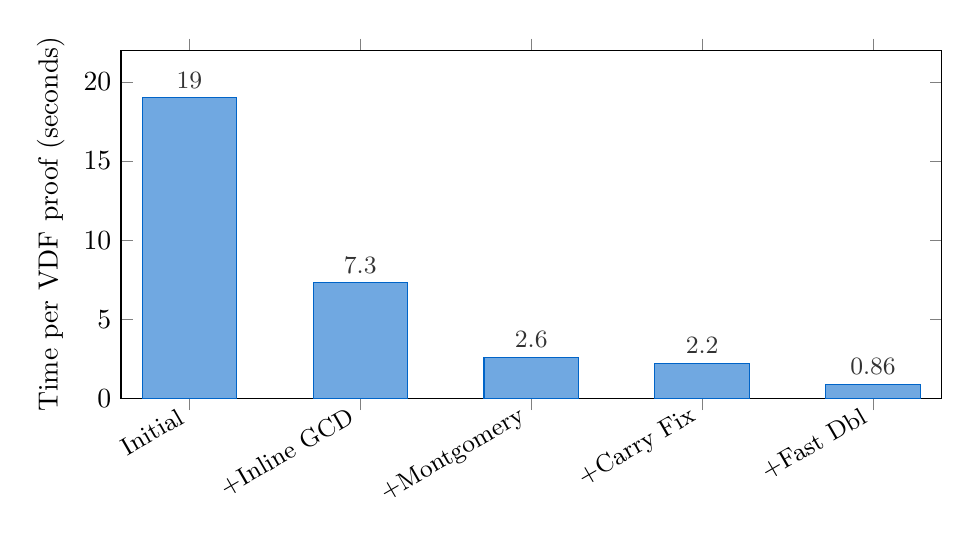
\begin{tikzpicture}
\begin{axis}[
    ybar,
    width=12cm,
    height=6cm,
    ylabel={Time per VDF proof (seconds)},
    symbolic x coords={Initial, +Inline GCD, +Montgomery, +Carry Fix, +Fast Dbl},
    xtick=data,
    x tick label style={rotate=30, anchor=east, font=\small},
    ymin=0,
    ymax=22,
    bar width=1.2cm,
    nodes near coords,
    nodes near coords style={font=\small, above},
    every axis plot/.append style={fill opacity=0.8},
]
\addplot[fill=qblue!70, draw=qblue] coordinates {
    (Initial, 19.0)
    (+Inline GCD, 7.3)
    (+Montgomery, 2.6)
    (+Carry Fix, 2.2)
    (+Fast Dbl, 0.86)
};
\end{axis}
\end{tikzpicture}
\end{center}

\begin{statbox}
\textbf{VDF Optimization Timeline}\\[5pt]
\begin{tabular}{@{}llrl@{}}
\toprule
\textbf{Optimization} & \textbf{Date} & \textbf{Per-Doubling} & \textbf{Speedup} \\
\midrule
Initial (BigInt mod) & Apr 14 & 4{,}400 $\mu$s & Baseline \\
Inline GCD + Proof Gen & Apr 15 & 1{,}700 $\mu$s & 2.6$\times$ \\
Montgomery CIOS & Apr 15 & 605 $\mu$s & 7.3$\times$ \\
CIOS Carry Bug Fix & Apr 15 & 521 $\mu$s & 8.4$\times$ \\
Fast Doubling Integration & Apr 15 & 200 $\mu$s & \textbf{22$\times$} \\
\bottomrule
\end{tabular}
\end{statbox}

\subsubsection{Montgomery CIOS Implementation}

The critical optimization was replacing arbitrary-precision \texttt{BigInt::mod\_floor()} division with fixed-width Montgomery multiplication using the CIOS (Coarsely Integrated Operand Scanning) method. For $p = 2^{256} - 189$:

\begin{itemize}
    \item Montgomery radix: $R = 2^{256}$, so $R \bmod p = 189$
    \item Precomputed: $R^2 \bmod p = 35{,}721$ and $-p^{-1} \bmod 2^{64}$
    \item Each multiplication: 4 limbs $\times$ 4 limbs with interleaved reduction
    \item \textbf{Key bug fix:} The CIOS carry propagation had a final reduction error that caused divergence after $\sim$256 sequential multiplications. Fixed by adding proper conditional subtraction after the accumulation loop.
\end{itemize}

\subsection{Dual-Lane Mining Protocol}

The dual-lane mining protocol splits block rewards 50/50 between BLAKE3 (GPU-friendly) and VDF (inherently sequential, CPU-fair) lanes.

\begin{center}
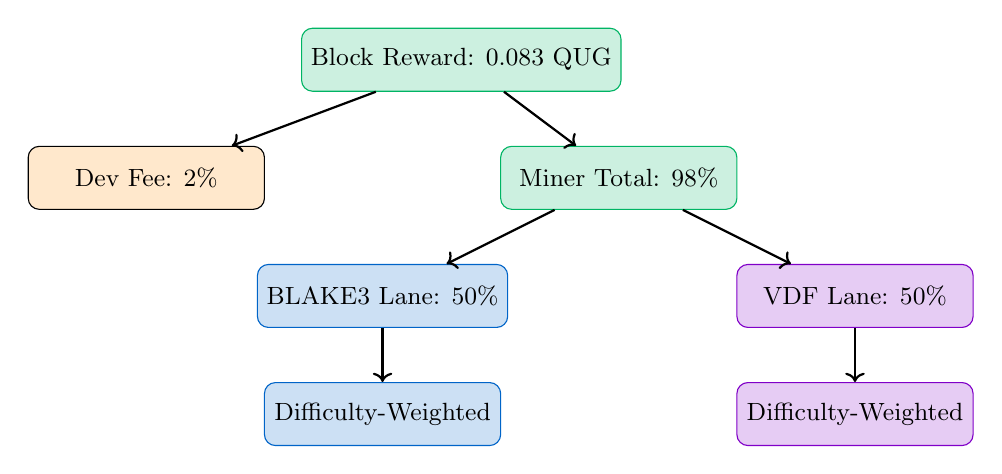
\begin{tikzpicture}[
    node distance=0.8cm,
    box/.style={draw, rounded corners, minimum width=3cm, minimum height=0.8cm, font=\small},
    blake/.style={box, fill=qblue!20, draw=qblue},
    vdf/.style={box, fill=qpurple!20, draw=qpurple},
    reward/.style={box, fill=qgreen!20, draw=qgreen},
]
    % Block reward flow
    \node[reward] (total) at (0,3) {Block Reward: 0.083 QUG};
    \node[box, fill=qorange!20] (dev) at (-4,1.5) {Dev Fee: 2\%};
    \node[reward] (miner) at (2,1.5) {Miner Total: 98\%};

    \node[blake] (b3) at (-1,0) {BLAKE3 Lane: 50\%};
    \node[vdf] (vdf) at (5,0) {VDF Lane: 50\%};

    \node[blake] (b3d) at (-1,-1.5) {Difficulty-Weighted};
    \node[vdf] (vdfd) at (5,-1.5) {Difficulty-Weighted};

    \draw[->, thick] (total) -- (dev);
    \draw[->, thick] (total) -- (miner);
    \draw[->, thick] (miner) -- (b3);
    \draw[->, thick] (miner) -- (vdf);
    \draw[->, thick] (b3) -- (b3d);
    \draw[->, thick] (vdf) -- (vdfd);
\end{tikzpicture}
\end{center}

\textbf{Conservation invariants} enforced in integer arithmetic:
\begin{align}
\texttt{blake3\_total} + \texttt{vdf\_total} &= \texttt{miner\_total} \\
\sum \texttt{blake3\_rewards}_i &= \texttt{blake3\_total} \\
\sum \texttt{vdf\_rewards}_i &= \texttt{vdf\_total} \\
\texttt{total\_reward} &= \texttt{dev\_fee} + \sum \texttt{all\_miner\_rewards}
\end{align}

The VDF lane is activated via a height-gated upgrade, ensuring zero behavioral change for existing miners before the activation height.

\subsection{q-flux Reverse Proxy}

Built from scratch in March 2026 to replace nginx on Epsilon after the connection pileup crisis. Key features:

\begin{center}
\begin{tabular}{@{}lp{8cm}@{}}
\toprule
\textbf{Feature} & \textbf{Description} \\
\midrule
Connection Pooling & Persistent upstream connections with configurable pool size per worker \\
Upstream Semaphore & 256 max in-flight requests per worker (48 workers $\times$ 256 = 12{,}288 global cap) \\
Health Auto-Recovery & Periodic health checks with automatic backend promotion/demotion \\
Super-Cluster Failover & Cross-node failover: Epsilon $\to$ Beta $\to$ Gamma $\to$ Delta \\
SSE Direct Bypass & Server-Sent Events bypass the proxy buffer for real-time streaming \\
Static File Serving & Efficient streaming of download binaries (no full buffering) \\
AIMD Concurrency & Additive-increase/multiplicative-decrease for upstream connection management \\
\bottomrule
\end{tabular}
\end{center}

\subsection{LWMA Difficulty Adjustment}

The Linearly Weighted Moving Average (LWMA) difficulty algorithm was activated at height 14{,}900{,}000 to regulate the uncontrolled 3.46 bps block rate toward the 1.0 bps target.

\begin{itemize}
    \item \textbf{Window:} 60 blocks with linear weights (1, 2, 3, \ldots, 60)
    \item \textbf{Solvetime clamp:} $[1\text{ms}, 6 \times \text{target}]$ per block
    \item \textbf{Adjustment clamp:} $[0.5\times, 2.0\times]$ per step
    \item \textbf{Floor:} 16 leading zero bits minimum
    \item \textbf{Bootstrap guard:} Requires $\geq$10 blocks before adjusting
\end{itemize}

\subsection{Checkpoint Sync}

New nodes cannot sync blocks 0--1{,}645{,}947 (the first 5 days of mainnet) because these blocks were deleted by a pruning bug that was fixed in v10.3.0. Checkpoint Sync solves this by:

\begin{enumerate}
    \item Detecting gaps via consecutive zero-block turbo sync responses
    \item Skipping forward in exponentially increasing steps to find where blocks begin
    \item Using HTTP probe (not P2P) to avoid race conditions with libp2p connection setup
    \item Preserving all balance data independently (mining rewards stored in separate column families)
\end{enumerate}

\subsection{HA Rolling Deployment Pipeline}

A zero-downtime deployment pipeline using 5 servers:

\begin{center}
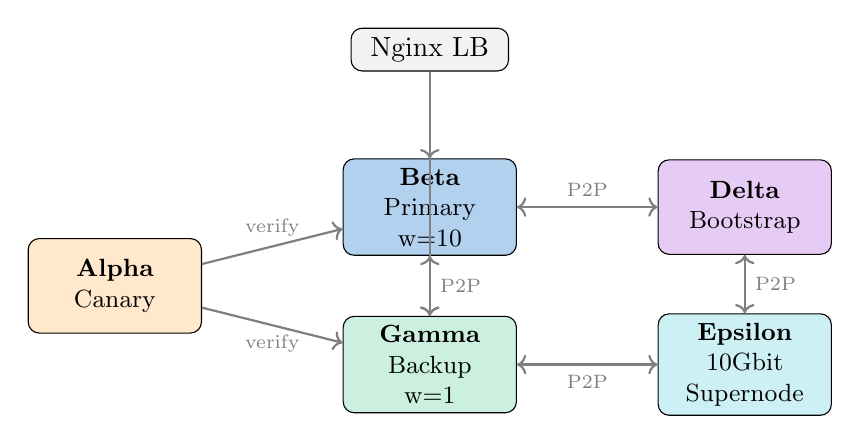
\begin{tikzpicture}[
    server/.style={draw, rounded corners, minimum width=2.2cm, minimum height=1.2cm, font=\small, align=center},
    arrow/.style={->, thick, gray},
]
    \node[server, fill=qorange!20] (alpha) at (0,0) {\textbf{Alpha}\\Canary};
    \node[server, fill=qblue!30] (beta) at (4,1) {\textbf{Beta}\\Primary\\w=10};
    \node[server, fill=qgreen!20] (gamma) at (4,-1) {\textbf{Gamma}\\Backup\\w=1};
    \node[server, fill=qpurple!20] (delta) at (8,1) {\textbf{Delta}\\Bootstrap};
    \node[server, fill=qcyan!20] (epsilon) at (8,-1) {\textbf{Epsilon}\\10Gbit\\Supernode};

    \draw[arrow] (alpha) -- node[above, font=\scriptsize]{verify} (beta);
    \draw[arrow] (alpha) -- node[below, font=\scriptsize]{verify} (gamma);
    \draw[arrow, <->] (beta) -- node[right, font=\scriptsize]{P2P} (gamma);
    \draw[arrow, <->] (beta) -- node[above, font=\scriptsize]{P2P} (delta);
    \draw[arrow, <->] (gamma) -- node[below, font=\scriptsize]{P2P} (epsilon);
    \draw[arrow, <->] (delta) -- node[right, font=\scriptsize]{P2P} (epsilon);

    % Nginx LB
    \node[draw, rounded corners, fill=gray!10, minimum width=2cm] (nginx) at (4,3) {Nginx LB};
    \draw[arrow] (nginx) -- (beta);
    \draw[arrow] (nginx) -- (gamma);
\end{tikzpicture}
\end{center}

\subsection{Additional Achievements}

\begin{center}
\begin{tabular}{@{}lll@{}}
\toprule
\textbf{Achievement} & \textbf{Date} & \textbf{Description} \\
\midrule
Crown Ash Game & Mar 28 & On-chain strategy game with siege mechanics, Bevy client \\
GPU Mining (OpenCL) & Mar 27 & BLAKE3 kernel for NVIDIA/AMD, adaptive work sizes \\
Windows Cross-Compile & Mar 25--28 & Full miner + node support for Windows (MinGW) \\
Dragon Ball FPGA & Apr 9--10 & Kintex-7 XC7K355T collaboration for ASIC mining \\
MCP Server & Apr 12 & Claude Code integration for wallet/mining operations \\
Slint Wallet Auto-Update & Mar 13 & Background check, download, SHA-256 verify, self-replace \\
Browser P2P Relay & Mar 30 & Browser-to-browser block relay via circuit relay \\
Starship Compute & Mar 8--10 & Distributed compute orchestrator (28 issues, all closed) \\
\bottomrule
\end{tabular}
\end{center}

% ============================================================================
% SECTION 5: ARCHITECTURE
% ============================================================================
\section{Infrastructure Architecture}

\subsection{Five-Server Topology}

\begin{center}
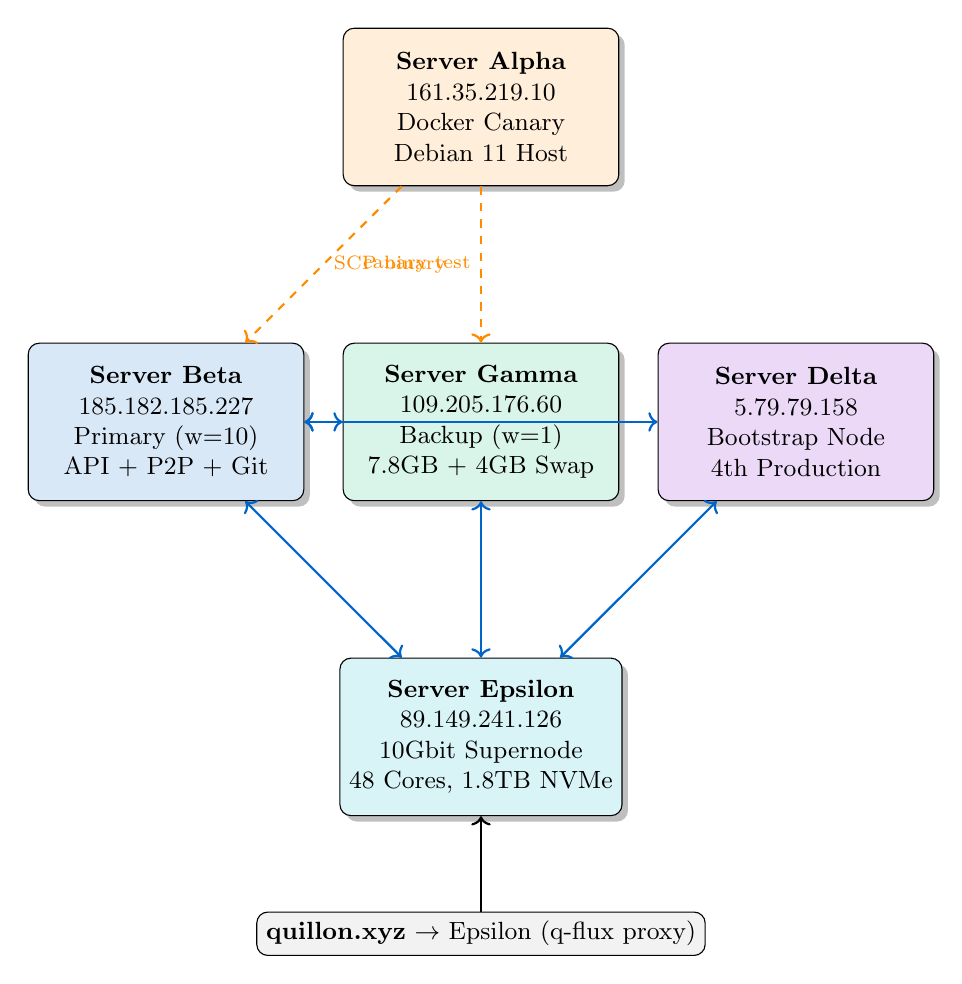
\begin{tikzpicture}[
    node distance=2cm,
    server/.style={draw, rounded corners, minimum width=3.5cm, minimum height=2cm, font=\small, align=center, drop shadow},
]
    % Servers
    \node[server, fill=qorange!15] (alpha) at (0,4) {
        \textbf{Server Alpha}\\
        161.35.219.10\\
        Docker Canary\\
        Debian 11 Host
    };

    \node[server, fill=qblue!15] (beta) at (-4,0) {
        \textbf{Server Beta}\\
        185.182.185.227\\
        Primary (w=10)\\
        API + P2P + Git
    };

    \node[server, fill=qgreen!15] (gamma) at (0,0) {
        \textbf{Server Gamma}\\
        109.205.176.60\\
        Backup (w=1)\\
        7.8GB + 4GB Swap
    };

    \node[server, fill=qpurple!15] (delta) at (4,0) {
        \textbf{Server Delta}\\
        5.79.79.158\\
        Bootstrap Node\\
        4th Production
    };

    \node[server, fill=qcyan!15] (epsilon) at (0,-4) {
        \textbf{Server Epsilon}\\
        89.149.241.126\\
        10Gbit Supernode\\
        48 Cores, 1.8TB NVMe
    };

    % Connections
    \draw[<->, thick, qblue] (beta) -- (gamma);
    \draw[<->, thick, qblue] (beta) -- (delta);
    \draw[<->, thick, qblue] (gamma) -- (epsilon);
    \draw[<->, thick, qblue] (delta) -- (epsilon);
    \draw[<->, thick, qblue] (beta) -- (epsilon);
    \draw[->, thick, qorange, dashed] (alpha) -- node[right, font=\scriptsize]{SCP binary} (beta);
    \draw[->, thick, qorange, dashed] (alpha) -- node[left, font=\scriptsize]{canary test} (gamma);

    % DNS
    \node[draw, rounded corners, fill=gray!10, font=\small] (dns) at (0,-6.5) {\textbf{quillon.xyz} $\to$ Epsilon (q-flux proxy)};
    \draw[->, thick] (dns) -- (epsilon);

\end{tikzpicture}
\end{center}

\subsection{Server Specifications}

\begin{center}
\begin{tabular}{@{}llllll@{}}
\toprule
& \textbf{Alpha} & \textbf{Beta} & \textbf{Gamma} & \textbf{Delta} & \textbf{Epsilon} \\
\midrule
Role & Canary & Primary & Backup & Bootstrap & Supernode \\
Bandwidth & --- & 100Mbit & 1Gbit & 1Gbit & \textbf{10Gbit} \\
RAM & --- & 16GB & 7.8GB+4GB swap & 8GB & 64GB \\
Cores & --- & 4 & 2 & 4 & \textbf{48} \\
Storage & Docker & SSD & SSD & SSD & \textbf{1.8TB NVMe} \\
Proxy & --- & Nginx & --- & --- & q-flux \\
\bottomrule
\end{tabular}
\end{center}

% ============================================================================
% SECTION 6: PERFORMANCE METRICS
% ============================================================================
\section{Performance Metrics}

\subsection{Network Statistics (April 15, 2026)}

\begin{center}
\begin{tabular}{@{}lr@{}}
\toprule
\textbf{Metric} & \textbf{Value} \\
\midrule
Network Height & 15{,}300{,}000+ blocks \\
Block Rate (pre-LWMA) & 3.37 blocks/second \\
Block Rate (post-LWMA target) & 1.0 blocks/second \\
Active Miners & 40+ \\
Peak Miners & 500+ (before LWMA) \\
Network Hash Rate & 11.38 GH/s \\
Total QUG Mined & 396{,}162 / 21{,}000{,}000 \\
Emission Rate & 2{,}625{,}000 QUG/year (Era 0) \\
Halving Period & 4 years \\
Wallet Addresses & 279 \\
DEX Liquidity Pools & 23 \\
Smart Contracts Deployed & 28 \\
Token Types & 1{,}913 balances tracked \\
\bottomrule
\end{tabular}
\end{center}

\subsection{Sync Performance}

\begin{center}
\begin{tabular}{@{}lrl@{}}
\toprule
\textbf{Phase} & \textbf{Speed} & \textbf{Notes} \\
\midrule
0--500K blocks & $\sim$280 blocks/sec & Warmup, peer discovery \\
500K--3M blocks & $\sim$1{,}100 blocks/sec & Peak turbo sync \\
Overall average & $\sim$570 blocks/sec & Full 11.4M block sync \\
Full sync time & $\sim$5.5 hours & On Epsilon (10Gbit) \\
\bottomrule
\end{tabular}
\end{center}

\subsection{VDF Performance (Release Mode)}

\begin{center}
\begin{tabular}{@{}lrl@{}}
\toprule
\textbf{Operation} & \textbf{Time} & \textbf{Notes} \\
\midrule
Single doubling & 200 $\mu$s & Montgomery CIOS, T=4300 \\
Full evaluation (T=4300) & 0.86 s & 4300 sequential doublings \\
Proof generation & $\sim$0.35 s & Wesolowski protocol \\
Total per VDF proof & $\sim$1.2 s & Eval + proof \\
Verification & $<$10 ms & Single exponentiation check \\
\bottomrule
\end{tabular}
\end{center}

\subsection{Version Progression}

\begin{center}
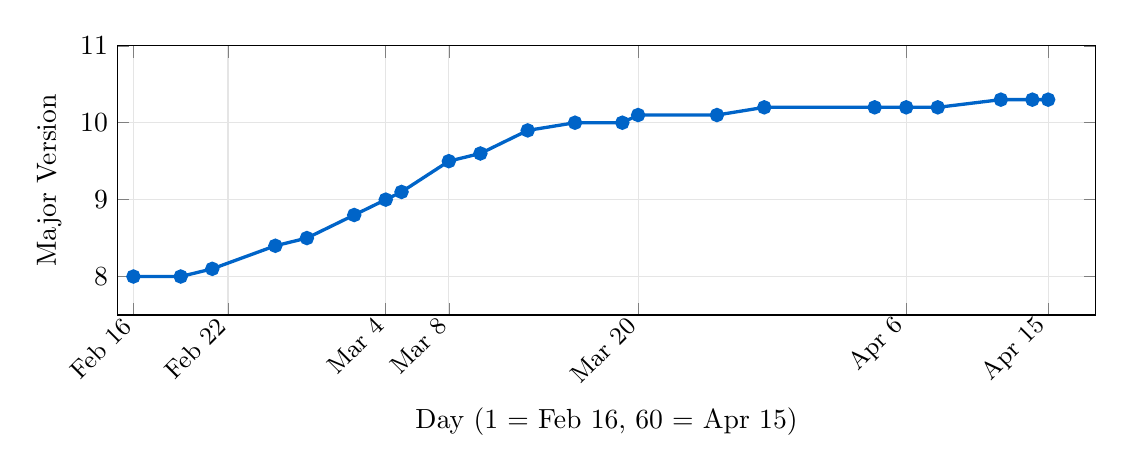
\begin{tikzpicture}
\begin{axis}[
    width=14cm,
    height=5cm,
    xlabel={Day (1 = Feb 16, 60 = Apr 15)},
    ylabel={Major Version},
    xmin=0, xmax=62,
    ymin=7.5, ymax=11,
    grid=both,
    grid style={gray!20},
    xtick={1, 7, 17, 21, 33, 50, 59},
    xticklabels={Feb 16, Feb 22, Mar 4, Mar 8, Mar 20, Apr 6, Apr 15},
    x tick label style={rotate=45, anchor=east, font=\small},
]
\addplot[qblue, very thick, mark=*] coordinates {
    (1, 8.0)
    (4, 8.0)
    (6, 8.1)
    (10, 8.4)
    (12, 8.5)
    (15, 8.8)
    (17, 9.0)
    (18, 9.1)
    (21, 9.5)
    (23, 9.6)
    (26, 9.9)
    (29, 10.0)
    (32, 10.0)
    (33, 10.1)
    (38, 10.1)
    (41, 10.2)
    (48, 10.2)
    (50, 10.2)
    (52, 10.2)
    (56, 10.3)
    (58, 10.3)
    (59, 10.3)
};
\end{axis}
\end{tikzpicture}
\end{center}

% ============================================================================
% SECTION 7: PROJECT MANAGEMENT
% ============================================================================
\section{Project Management}

\subsection{Risk Matrix}

\begin{center}
\begin{tabular}{@{}p{3cm}llp{4.5cm}@{}}
\toprule
\textbf{Risk} & \textbf{Likelihood} & \textbf{Impact} & \textbf{Mitigation} \\
\midrule
Balance corruption & Medium & Critical & Triple-redundant storage (RocksDB, HTTP state sync, P2P gossipsub) \\
Node OOM crash & High & High & RocksDB cache caps, semaphore-gated allocations, jemalloc tuning \\
Network partition & Low & Critical & 5-server topology with gossipsub mesh \\
Sync-down attack & Medium & Critical & Application + database layer safety checks \\
Consensus fork & Low & Critical & Height-gated upgrades via Consensus Guard \\
Single point of failure & Medium & High & HA rolling deploy, q-flux cluster failover \\
Pruning data loss & Low (fixed) & High & Pruning disabled; checkpoint sync for gaps \\
\bottomrule
\end{tabular}
\end{center}

\subsection{Resource Allocation}

\begin{center}
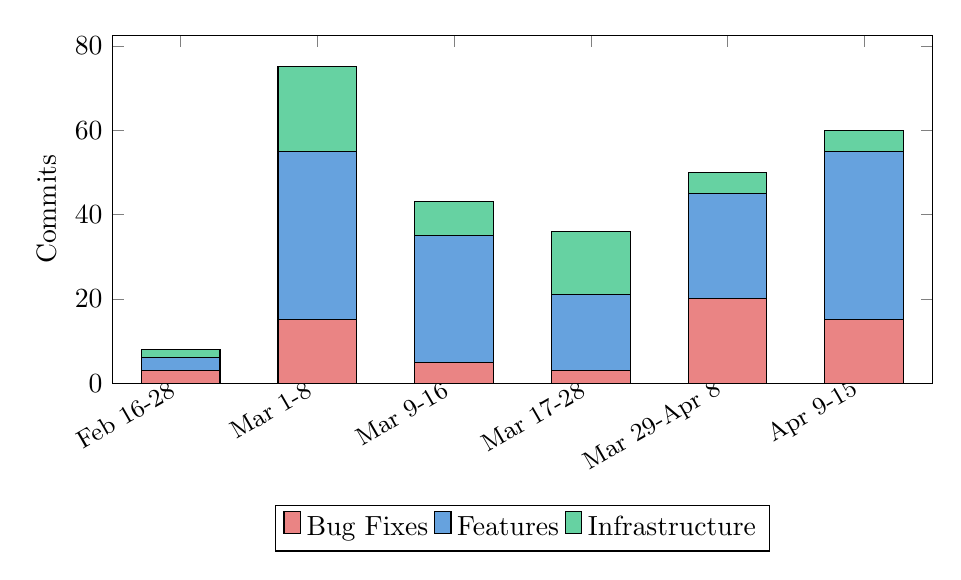
\begin{tikzpicture}
\begin{axis}[
    ybar stacked,
    width=12cm,
    height=6cm,
    ylabel={Commits},
    symbolic x coords={Feb 16-28, Mar 1-8, Mar 9-16, Mar 17-28, Mar 29-Apr 8, Apr 9-15},
    xtick=data,
    x tick label style={rotate=30, anchor=east, font=\small},
    ymin=0,
    bar width=1cm,
    legend style={at={(0.5,-0.35)}, anchor=north, legend columns=3},
]
\addplot[fill=qred!60] coordinates {
    (Feb 16-28, 3) (Mar 1-8, 15) (Mar 9-16, 5) (Mar 17-28, 3) (Mar 29-Apr 8, 20) (Apr 9-15, 15)
};
\addplot[fill=qblue!60] coordinates {
    (Feb 16-28, 3) (Mar 1-8, 40) (Mar 9-16, 30) (Mar 17-28, 18) (Mar 29-Apr 8, 25) (Apr 9-15, 40)
};
\addplot[fill=qgreen!60] coordinates {
    (Feb 16-28, 2) (Mar 1-8, 20) (Mar 9-16, 8) (Mar 17-28, 15) (Mar 29-Apr 8, 5) (Apr 9-15, 5)
};
\legend{Bug Fixes, Features, Infrastructure}
\end{axis}
\end{tikzpicture}
\end{center}

\subsection{Deployment Frequency}

During this period, the project averaged \textbf{4.2 commits per day} and performed approximately \textbf{50 production deployments} using the HA rolling deploy pipeline. No deployment caused user-visible downtime.

% ============================================================================
% SECTION 8: LESSONS LEARNED
% ============================================================================
\section{Lessons Learned}

\subsection{From Critical Incidents}

\begin{enumerate}[leftmargin=*, label=\textbf{L\arabic*.}]
    \item \textbf{Never use \texttt{saturating\_sub} in financial code.} The balance reorg handler silently zeroed accounts because \texttt{saturating\_sub} clamps to zero instead of signaling an error. Financial arithmetic must use checked operations that fail loudly.

    \item \textbf{Lock contention is invisible until it cascades.} The mining endpoint write lock worked fine with 10 miners. At 500 miners, the queuing cascade created 38K connections in minutes. Non-blocking \texttt{try\_lock} with cached fallback is mandatory for high-concurrency endpoints.

    \item \textbf{Ephemeral port ranges can collide with service ports.} The TCP self-connection bug on Epsilon (port 8080 in the ephemeral range) was diagnosed only by examining \texttt{ss -tan} output. Always verify service ports are outside \texttt{ip\_local\_port\_range}.

    \item \textbf{Unbounded \texttt{tokio::spawn} is a memory bomb.} Each syncing peer requesting 500+ blocks via block-pack could allocate 50--150MB. Without a semaphore, 10GB+ allocations crashed Epsilon 6+ times per hour.

    \item \textbf{Aggressive pruning on a live chain deletes history permanently.} The pruning bug deleted blocks 0--1.6M (the first 5 days of mainnet). Pruning must never run without explicit operator consent and a confirmed checkpoint.

    \item \textbf{\texttt{kill -9} on a database node creates corrupt blocks that look valid.} After a forced kill, 180 blocks had partial writes that passed key-existence checks but failed deserialization. Gap detection must use deserialization, not just key lookup.

    \item \textbf{Constants must be verified by counting zeros.} The emission controller bug (3 extra zeros, 34$\times$ overshoot) was caught by unit tests but could have been caught earlier by a code review policy requiring comments that spell out the full numeric value.

    \item \textbf{Build caches lie.} After changing genesis timestamp constants, Cargo's incremental compilation reused stale object files. Always \texttt{cargo clean --package} after changing constants.

    \item \textbf{Triple redundancy saved the project.} Balance data survived every crisis because it is stored in three independent locations: RocksDB column families, HTTP state sync snapshots, and P2P gossipsub propagation.

    \item \textbf{18-hour debugging sessions find more bugs than 18 one-hour sessions.} The emergency session on April 13--14 found 5 interconnected bugs that only manifested under specific combinations of reorg + DEX swap + restart conditions.
\end{enumerate}

% ============================================================================
% SECTION 9: ROADMAP
% ============================================================================
\section{Roadmap: Q2--Q3 2026}

\begin{futurebox}
\textbf{Q2 2026 (April--June): Stabilization and CPU Fairness}

\begin{enumerate}
    \item \textbf{VDF Mining Launch}
    \begin{itemize}
        \item Deploy dual-lane mining to mainnet (Phase C activation)
        \item Montgomery CIOS performance tuning (target: 100$\mu$s/doubling)
        \item VDF miner binary distribution (Linux + Windows)
    \end{itemize}

    \item \textbf{Chain Rebuild}
    \begin{itemize}
        \item Fix \texttt{rebuild\_balances\_from\_chain()} crash (P0 from emergency session)
        \item Ensure balances can be independently verified from block data
        \item Eliminate dependency on authority node for balance truth
    \end{itemize}

    \item \textbf{Memory Optimization}
    \begin{itemize}
        \item Jemalloc per-arena purge (fix 35--52GB RSS fragmentation)
        \item SparseMerkleTrie cache bounded to 500K entries
        \item RocksDB compaction tuning for long-running nodes
    \end{itemize}

    \item \textbf{Dragon Ball FPGA/ASIC}
    \begin{itemize}
        \item RTL verification for BLAKE3 chain semantics
        \item Scratchpad integration for Kintex-7 XC7K355T
        \item Testnet mining with hardware prototypes
    \end{itemize}
\end{enumerate}
\end{futurebox}

\begin{futurebox}
\textbf{Q3 2026 (July--September): Scale and Ecosystem}

\begin{enumerate}
    \item \textbf{Network Scaling}
    \begin{itemize}
        \item Target: 100+ concurrent miners with sub-second block propagation
        \item Sharded gossipsub for reduced bandwidth per node
        \item Geographic node distribution incentives
    \end{itemize}

    \item \textbf{Ecosystem Growth}
    \begin{itemize}
        \item Crown Ash game: phases 3--5 (siege mechanics, world events)
        \item DEX v2: order book mode alongside AMM
        \item Ethereum bridge: production deployment with Reth integration
        \item Mobile wallet: production release for iOS/Android
    \end{itemize}

    \item \textbf{Security Hardening}
    \begin{itemize}
        \item External security audit engagement
        \item Formal verification of balance conservation invariants
        \item SQIsign post-quantum signature integration (replacing scaffold)
    \end{itemize}
\end{enumerate}
\end{futurebox}

% ============================================================================
% SECTION 10: CONCLUSION
% ============================================================================
\section{Conclusion}

The February--April 2026 period represents the most consequential two months in Quillon Graph's history. The project launched its mainnet, survived 11 critical incidents without permanent data loss, and delivered breakthrough innovations in CPU-fair mining through the Genus-2 Jacobian VDF.

The 253 commits across this period reflect a development intensity driven by the realities of operating a live, \$1B-market-cap blockchain. Every crisis---from the 38K connection pileup to the 18-hour emergency balance session---produced architectural improvements that made the system more resilient.

Key metrics tell the story: 15.3 million blocks produced, 396{,}162 QUG mined, 40+ active miners, and a 22$\times$ VDF performance improvement from initial implementation to Montgomery-optimized production code.

The dual-lane mining protocol, combining GPU-friendly BLAKE3 with inherently-sequential VDF proofs, represents a novel approach to the GPU centralization problem that plagues most proof-of-work systems. By guaranteeing that 50\% of mining rewards are accessible only through sequential computation, Quillon Graph ensures that CPU miners remain economically viable regardless of GPU hashrate concentration.

Looking forward, the priorities are clear: complete the VDF mining deployment, fix the chain rebuild function to eliminate authority-node dependency, and engage external security auditors before the next growth phase. The infrastructure is battle-tested. The architecture is proven. The path from crisis to innovation continues.

\vspace{1cm}
\begin{center}
\textit{``Every crisis we survived made the system stronger. Every bug we fixed protected real value. Every optimization we shipped proved that CPU-fair mining is not just possible---it is inevitable.''}
\end{center}

% ============================================================================
% APPENDIX
% ============================================================================
\appendix

\section{Version Changelog Summary}

\begin{longtable}{@{}llp{8cm}@{}}
\toprule
\textbf{Version} & \textbf{Date} & \textbf{Key Changes} \\
\midrule
\endhead
v8.0.0 & Feb 19 & Mainnet preparation: 23 crate updates, bounty migration, MCP, AI chat \\
v8.1.3 & Feb 21 & DEX fixes, SMTP, TUI, balance safety \\
v8.4.2 & Feb 25 & Deterministic balance consensus, XLIST campaigns \\
v8.5.9 & Feb 27 & Miner version fix, QCredit vault \\
v8.8.0 & Mar 2 & Dune Analytics pipeline, Epsilon deployment \\
v8.9.5 & Mar 3 & Zero-drop mining queue \\
v8.9.8 & Mar 4 & Non-blocking challenge lock (38K connection fix) \\
v9.0.1 & Mar 4 & Miner bandwidth: 111 KB/s $\to$ 2--5 KB/s \\
v9.1.3 & Mar 5 & Mining perf fix, deploy panel \\
v9.2.5 & Mar 7 & q-flux super-cluster failover \\
v9.3.1 & Mar 8 & K-parameter gauge with zk-STARK privacy \\
v9.5.0 & Mar 8 & Starship Endgame compute orchestrator \\
v9.8.0 & Mar 12 & SharkGod transaction beam \\
v9.9.1 & Mar 13 & Command Center water robot swarm \\
v10.0.2 & Mar 15 & Miner bandwidth reduction \\
v10.0.8 & Mar 18 & Windows sync fix (rustls-tls) \\
v10.1.4 & Mar 25 & Mobile wallet, GPU mining refactor, Ethereum bridge \\
v10.1.8 & Mar 27 & GPU: async dispatch, kernel cache, per-GPU adaptive \\
v10.2.1 & Mar 28 & Crown Ash game integration \\
v10.2.6 & Apr 4 & Zero-downtime mining supercluster, Genus-2 VDF wiring \\
v10.2.8 & Apr 6--7 & Corrupt block recovery, turbo sync fixes \\
v10.2.9 & Apr 8--10 & Height atomic stall, block-pack I/O, log spam reduction \\
v10.3.0 & Apr 12--13 & LWMA difficulty, pruning fix, MCP server, crypto dashboard \\
v10.3.2 & Apr 14 & EMERGENCY: disable reorg handler, DEX double-deduction fix \\
v10.3.3 & Apr 14 & Plan B: Beta authority balance sync to all 274 wallets \\
v10.3.4 & Apr 14 & Genus-2 VDF dual-lane mining, standalone VDF miner \\
v10.3.5 & Apr 15 & Montgomery 19$\times$ speedup, Checkpoint Sync \\
\bottomrule
\end{longtable}

\section{Commit Distribution by Category}

\begin{center}
\begin{tabular}{@{}lr@{}}
\toprule
\textbf{Category} & \textbf{Count} \\
\midrule
Features (\texttt{feat}) & 128 \\
Bug Fixes (\texttt{fix}) & 72 \\
Performance (\texttt{perf}) & 11 \\
Documentation (\texttt{docs}) & 18 \\
Tests (\texttt{test}) & 8 \\
Infrastructure (\texttt{chore}) & 8 \\
Debug Instrumentation (\texttt{debug}) & 8 \\
\midrule
\textbf{Total} & \textbf{253} \\
\bottomrule
\end{tabular}
\end{center}

\end{document}
